%%%%%%%%%%%%%%%%%%%%%%%%%%%%%%%%%%%%%%%%%%%%%%%%%%%%%%%%%%%%%%%%%%%%%%%%
% Escuela Politécnica Superior de la Universidad de Alicante
% Realizado por: Jose Manuel Requena Plens
% Contacto: info@jmrplens.com / Telegram:@jmrplens
%%%%%%%%%%%%%%%%%%%%%%%%%%%%%%%%%%%%%%%%%%%%%%%%%%%%%%%%%%%%%%%%%%%%%%%%

\definecolor{mycolor1}{rgb}{1.00000,0.00000,1.00000}%
%
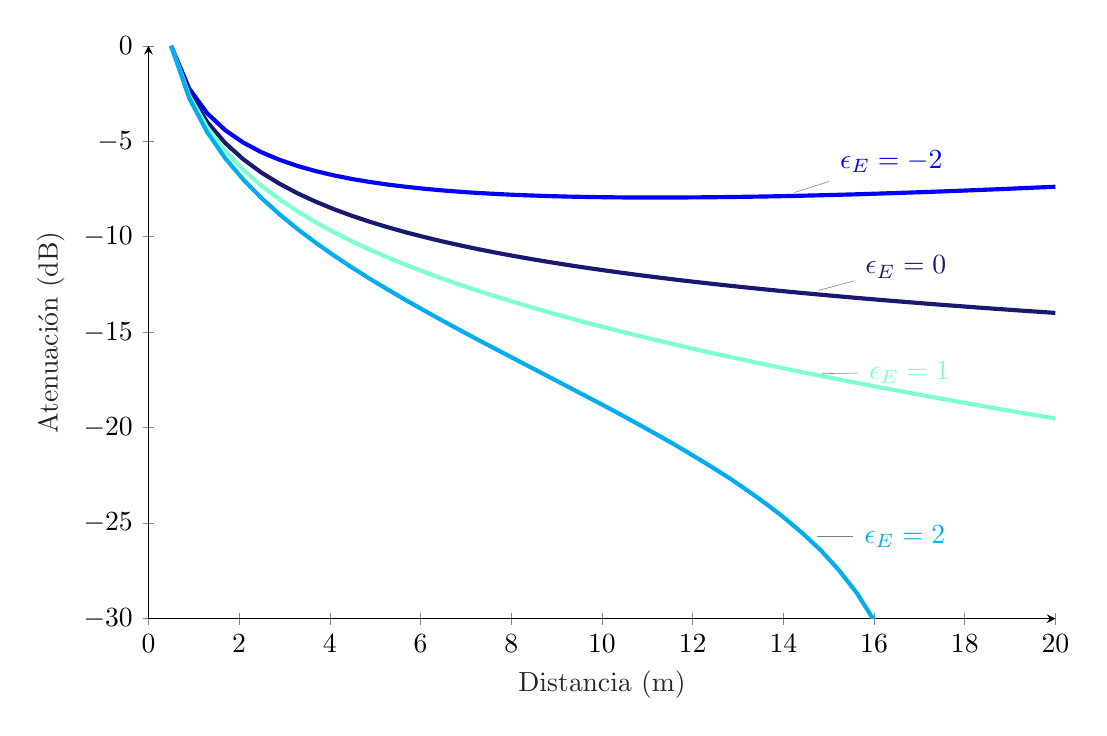
\begin{tikzpicture}

\begin{axis}[%
width=0.95\textwidth,
height=0.6\textwidth,
at={(0\textwidth,0\textwidth)},
scale only axis,
xmin=0,
xmax=20,
xlabel style={font=\color{white!15!black}},
xlabel={Distancia (m)},
ymin=-30,
ymax=0,
axis y line=left,
axis x line=bottom,
ylabel style={font=\color{white!15!black}},
ylabel={Atenuación (dB)},
axis background/.style={fill=white},
legend style={legend cell align=left, align=left, draw=white!15!black}
]



\addplot [color=blue, line width=1.5pt,domain=0.5:20, samples=50]
{10*ln(1.0337e+12*((3.5407e-04/x)* ( e^(-(13.82*(x/343)*(-2)/1.2098)) - e^(-(13.82*(x/343+0.05)*1/1.2098)))))/ln(10) - 10*ln(1.0337e+12*((3.5407e-04/0.5)* ( e^(-(13.82*(0.5/343)*(-2)/1.2098)) - e^(-(13.82*(0.5/343+0.05)*1/1.2098)))))/ln(10)} node [pos=0.75,pin=15:{$\epsilon_E=-2$}] {};

\addplot [color=MidnightBlue, line width=1.5pt,domain=0.5:20, samples=50]
{10*ln(1.0337e+12*((3.5407e-04/x)* ( e^(-(13.82*(x/343)*(0)/1.2098)) - e^(-(13.82*(x/343+0.05)*1/1.2098)))))/ln(10) - 10*ln(1.0337e+12*((3.5407e-04/0.5)* ( e^(-(13.82*(0.5/343)*(0)/1.2098)) - e^(-(13.82*(0.5/343+0.05)*1/1.2098)))))/ln(10)} node [pos=0.79,pin=5:{$\epsilon_E=0$}] {};

\addplot [color=Aquamarine, line width=1.5pt,domain=0.5:20, samples=50]
{10*ln(1.0337e+12*((3.5407e-04/x)* ( e^(-(13.82*(x/343)*(1.1)/1.2098)) - e^(-(13.82*(x/343+0.05)*1/1.2098)))))/ln(10) - 10*ln(1.0337e+12*((3.5407e-04/0.5)* ( e^(-(13.82*(0.5/343)*(1.1)/1.2098)) - e^(-(13.82*(0.5/343+0.05)*1/1.2098)))))/ln(10)} node [pos=0.80,pin=2:{$\epsilon_E=1$}] {};

\addplot [color=cyan, line width=1.5pt,domain=0.5:20, samples=50]
{10*ln(1.0337e+12*((3.5407e-04/x)* ( e^(-(13.82*(x/343)*(2)/1.2098)) - e^(-(13.82*(x/343+0.05)*1/1.2098)))))/ln(10) - 10*ln(1.0337e+12*((3.5407e-04/0.5)* ( e^(-(13.82*(0.5/343)*(2)/1.2098)) - e^(-(13.82*(0.5/343+0.05)*1/1.2098)))))/ln(10)} node [pos=0.74,pin=0:{$\epsilon_E=2$}] {};

\end{axis}
\end{tikzpicture}%